\subsection{Introduction}
This approach avoid treating parameters like random variables, and which thus avoid the 
use of priors and Bayes rule.


\subsection{Sampling distribution of an estimator}
In frequentist statistic a parameter estimate $\hat{\theta}$ is computed by applying an
estimator $\delta$ to some data $\mathcal{D}$, so $\hat{\theta}=\delta(\mathcal{D})$.
The uncertainty in the parameter estimate can be measured by computing the \emph{sampling
distribution} of the estimator.
Imagine sampling many different datasets $\mathcal{D}^{(s)}$ from some true model 
$p(\cdot|\theta^{*})$ meaning $\mathcal{D}^{(s)}=\left\{x_{i}^{(s)}\hookrightarrow 
p(\cdot|\theta^{*})\right\}_{1\leq i\leq N}$ for $1\leq s\leq S$ and $\theta^{*}$ is the 
true parameter. Now apply the estimator $\hat{\theta}(\cdot)$ to each $\mathcal{D}^{(s)}$
to get a set of estimates $\{\hat{\theta}(\mathcal{D}^{(s)})\}_{1\leq s\leq S}$.\\
As we late $S \rightarrow \infty$, the distribution induced on $\hat{\theta}(\cdot)$ is 
the \textbf{sampling distribution of the estimator}.

\paragraph{Bootstrap}
It is a simple \emph{Monte Carlo} technique to approximate the sampling 
distribution.
The idea is that if we knew the true parameters $\theta^{*}$, we could generate $S$ fake 
datasets of size $N$, from the true distribution. We could then compute our estimator from
each sample, and use the empirical distribution of the resulting samples as our estimate
of the sampling distribution.\\
Since $\theta$ is unknown, the idea of the \textbf{parametric bootstrap} is to generate
the samples using $\hat{\theta}(\mathcal{D})$ instead.
An alternative, called \textbf{non-parametric bootstrap} is to sample the $x_{i}^{s}$
(with replacement) from the original data $\mathcal{D}$ and then compute the induced
distribution as before.

\subsection{Fequentist decision theory}
In Frequentist decision theory there is a loss function and a likelihood, but there
is no prior and hence no posterior or posterior expected loss. Thus there is no 
automatic way of deriving an optimal estimator, unlike the Bayesian case.\\
Instead, we are free to choose any estimator or decision procedure $\delta: \mathcal{X}
\rightarrow \mathcal{A}$ we want.\\
Having chosen an estimator, we define its expected loss or risk as follows
\begin{center}
 $R(\theta^{*}, \delta) \triangleq \mathbb{E}_{p(\tilde{\mathcal{D}}|\theta^{*})}
\left(L(\theta^{*}, \delta(\tilde{\mathcal{D}}))\right) = \Su{}{}L\left(\theta^{*},
\delta(\tilde{\mathcal{D}})p(\tilde{\mathcal{D}})\right)d\tilde{\mathcal{D}}$   
\end{center}
where $\tilde{\mathcal{D}}$ is data sampled from 'nature's distribution' which is 
represented by parameter $\theta^{*}$.
Whereas the Bayesian posterior expected loss: 
\begin{center}
    $p(a, \mathcal{D, \pi}) \triangleq \mathbb{E}_{p(\theta|\mathcal{D},\pi)}\left(
        L(\theta, a) = \Su{\Theta}{}L(\theta, \bm{a})p(\theta|\mathcal{D}, \pi)d\theta
    \right)$
\end{center}
We see that the Bayesian approach averages over $\theta$, which is unknown, and conditions
on $\mathcal{D}$ which is known. Unlike the frequentist approach averages over $\tilde{
\mathcal{D}}$, thus ignoring the observed data, and conditions on $\theta^{*}$ which is 
unknown.

\paragraph{Bayes risk}
How to chose amongst the estimators? 
We need some way to convert $R(\theta^{*}, \delta)$ into single measure of quality, $R(
\delta)$ which does not depend on knowing $\theta^{*}$. One approach is to put a prior on
$\theta^{*}$ and then to define \textbf{Bayes risk} of an estimator as follows:
\begin{center}
    $R_{B}(\delta) \triangleq \mathbb{E}_{p(\theta^{*})}\left(R(\theta^{*}, \delta)\right)
    \Su{}{}R(\theta^{*}, \delta)p(\theta^{*})d\theta^{*}$
\end{center}
A \textbf{Bayes estimator} or \textbf{Bayes decision rule} is one which minimizes the 
expected risk: $\delta_{B} \triangleq \displaystyle\argmin_{\delta} R_{B}(\delta)$
\subparagraph{Connection Bayesian and Frequentist approaches to decision theory.}
\begin{itemize}
    \item \emph{Theorem 1} A Bayes estimator can be optained by minimizing the posterior 
        expected loss for each $\bm{x}$
    \item \emph{Theorem 2} Every admissible decision rule is a Bayes decision rule with 
        respect to some possibly improper prior distribution.
\end{itemize}
\subparagraph{Minimax risk}
Some frequentist statistic users avoid using Bayes risk since it requires the choice of
a prior, although this is only in the evaluation of the estimator, not necessarily as 
part of its construction. An alternative approach is as follows:
\begin{enumerate}
    \item Define the  maximum risk of an estimator as:\\
        $R_{max}(\delta) \triangleq \displaystyle\theta^{*}R(\bm{\theta}^{*},\delta)$
    \item A \textbf{minimax rule} is one which minimizes the maximum risk:
        $\delta_{MM} \triangleq \displaystyle\argmin_{\delta} R_{\max}(\delta)$
\end{enumerate}
Minimax estimators have a certain appeal, however computing them can be hard and 
furthermore they are very pessimistic.
In most statistical situations, excluding games theoretic ones, assuming nature is an
adversary is not a reasonable assumption.
\subparagraph{Admissible estimators}
The basic problem with frequentis decision theory is that it relies on knowing the true
distribution $p(\cdot|\theta^{*})$ in order to evaluate the risk. However it might be 
the case that some estimators are worse than others regardless of the value of 
$\theta^{*}$.\\
In particular if for $\theta \in \Theta, R(\theta, \delta_{1}) \leq R(\theta, \delta_{2})$
then we say that $\delta_{1}$ \textbf{dominates} $\delta_{2}$.\\
An estimator is said to be \textbf{admissible} if it is not strictly dominated by any 
other estimator.\\
\textbf{Admissibility is not enough}


\subsection{Desirable properties of estimators}
\subparagraph{Consistent estimators}
An estimator is said to be \textbf{consistent} if it eventually recovers the true
parameters that generated the data as the sample size goes to infinity. 

\subparagraph{Unbiased estimator}
The \textbf{bias} of an estimator is defined as 
\begin{center}
    $bias\left(\hat{\theta}(\cdot)\right) = \mathbb{E}_{p(\mathcal{D}|\theta^{*})}
    \left(\hat{\theta}(\mathcal{D})-\theta^{*}\right)$
\end{center}
The estimator is unbiased when the bias is equal to 0.

\subparagraph{Minimum variance estimators}
A famous result called the \textbf{Cramerè-Rao lower bound} provides a lower bound on the
variance of any unbiased estimator. More precisely:
Let $\left(X_{j}\right)_{1 \leq j \leq p} \hookrightarrow p(X|\theta_{0})$ and 
$\hat{\theta}(\cdot)$ an unbiased estimator of $\theta^{*}$
Then, under various smoothness assumptions on $p(X|\theta_{0})$ we have  
\begin{center}
    $\mathbb{V}(\hat{\theta}) \geq \dfrac{1}{nI(\theta^{*})}$
\end{center}
where $I(\theta^{*})$ is the Fisher information matrix.

\subparagraph{Bias-Variance Trade-off} 
As $MSE = variance + bias^{2}$\\
It might be wise to use a biased estimator, so long as it reduces our variance, assuming
our goal is to minimize squared error. 


\subsection{Empirical risk minimization}
Frequentist decision theory suffers from the fundamental problem that one cannot actually
compute the risk function, since it relies on knowing the true data distribution. By
contrast, the Bayesian posterior expected loss can always be computed since it conditions
on the data rather that on $\theta^{*}$.\\
However there is one setting which avoids this problem, it is when the task is to predict
observable quantities, as opposed to estimating hidden variables or parameters.\\
Instead of looking at loss functions of the form $L(\bm{\theta^{*}}, \delta(\mathcal{D}))$
let us look at loss functions of the form $L(y, \delta(\bm{x}))$.\\
Then the risk becomes:
$R(p_{*}, \delta) \triangleq \mathbb{E}_{(\bm{x}, y)\hookrightarrow p_{*}}\left(L(y,
\delta(\bm{x}))\right) = \su{\bm{x}}{}\su{\bm{y}}{}L(y, \delta(\bm{x}))p_{*}(\bm{x}, y)$
Where $p_{*}$ represents "nature's distribution", indeed this distribution is unknown, 
but a simple approach is to use the empirical distribution, derived from some training 
data to approximate $p_{*}$
$p_{emp} \triangleq \dfrac{1}{N}\su{i=1}{N}\delta_{x_{i}}(\bm{x})\delta_{y_{i}}(y) 
\approx p_{*}(\bm{x}, y)$
We define the empirical risk as follows:
\begin{center}
    $R_{emp}(\mathcal{D}, \mathcal{D}) \triangleq R(p_{emp}, \delta) = \dfrac{1}{N}
    \su{i=1}{N}L(y_{i}, \delta(x_{i}))$
\end{center}
\suparagraph{Regularized risk minimization}
\begin{center}
    $R'(\mathcal{D}, \delta) = R_{emp}(\mathcal{D}, \delta) + \lambda C(\delta)$
\end{center}
where $C(\delta)$ measures the complexity of the prediction function $\delta(\bm{x})$ and 
$\lambda$ controls the strength of the complexity penalty. 
This approach is known as \textbf{regularized risk minimization}.

\paragraph{Estimating the risk using cross validation}
Principle of cross validation













\subsection{Tools}
\paragraph{Introduction}
Avoid treating parameters as randome variables.
The notion of variation across repeated trials forms the basis for modelling
uncertainity.


\paragraph{Hypothesis Testing}
A \emph{frequentist} statistics, probabilities represent the frequencies at which 
particular events happen.

\paragraph{\emph{p-value}}
It is the heart of frequentist hypothesis testing, it tells us the probability of getting
a particular test statistic $t$ as big as the one we have or bigger under the null 
hypothesis (that there is actually no effect).\\
By convention we usually conclude an effect is \emph{statistically significant} if the 
\emph{p-value} is less than a threshold $\alpha$.

\paragraph{Confidence intervals}
When we fit a model to our data we look for the \emph{maximum of likelihood} parameters,
meaning the parameters that are most consistent with our data. 
For each parameter we will able to construct $95\%$ interval namely $95$ of the $100$ 
intervals generated will contain the true value of the parameter.\\
If $H_{0}: \beta=0$ is true, the probability of getting a $95\%$ confidence interval that
does not include 0 is less than 0.05. In other words, if the $95\%$ confidence does not 
include 0, $p<0.05$.
\begin{figure}[H]
	\begin{center}
		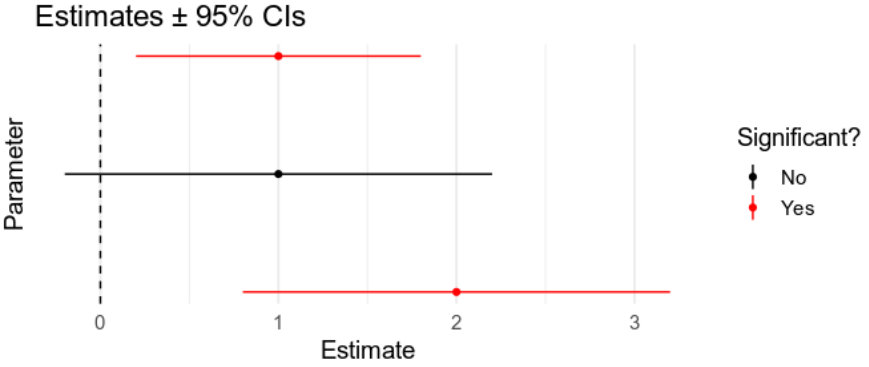
\includegraphics[width=\textwidth]{./chaps/10sec/images/4_estimates.png}
	\end{center}
	\caption{Confidence interval}
	\label{fig:4_estimates}
\end{figure}

\paragraph{Multiple comparisons}
The more tests we run the more likely it is to we'll find at least one that is significant
even though the null hypothesis is true. We can then apply a Bonferroni correction.\\
Let's say we are running $k$ tests, we can either adjust: 
\begin{itemize}
	\item the threshold $\alpha_{adj} = \dfrac{\alpha}{k}$ OR
	\item the \emph{p-value} $p_{ajd} = k\times p$
\end{itemize}
